%\chapter{New Ultrashort X-ray Sources}
\chapter{X-ray Lasers}
\label{Ultrashort X-ray Sources}\noindent
 
Since the discovery of X-rays by Wilhelm R\"{o}ntgen in 1895 X-ray sources have
continuously improved, often leading to significant new science. The increase in
brilliance since the first rotating anodes used for crystallography has been
spectacular, bridging many orders of magnitude. The development of dedicated
synchrotron light sources in the beggining of the 80s contributed to an explosion of
protein structures solved by crystallography. A further boost came with
the introduction of wigglers, undulators and the increase in brightness from
third generation sources, which employ them.

 
\begin{figure}[h]
\centering
  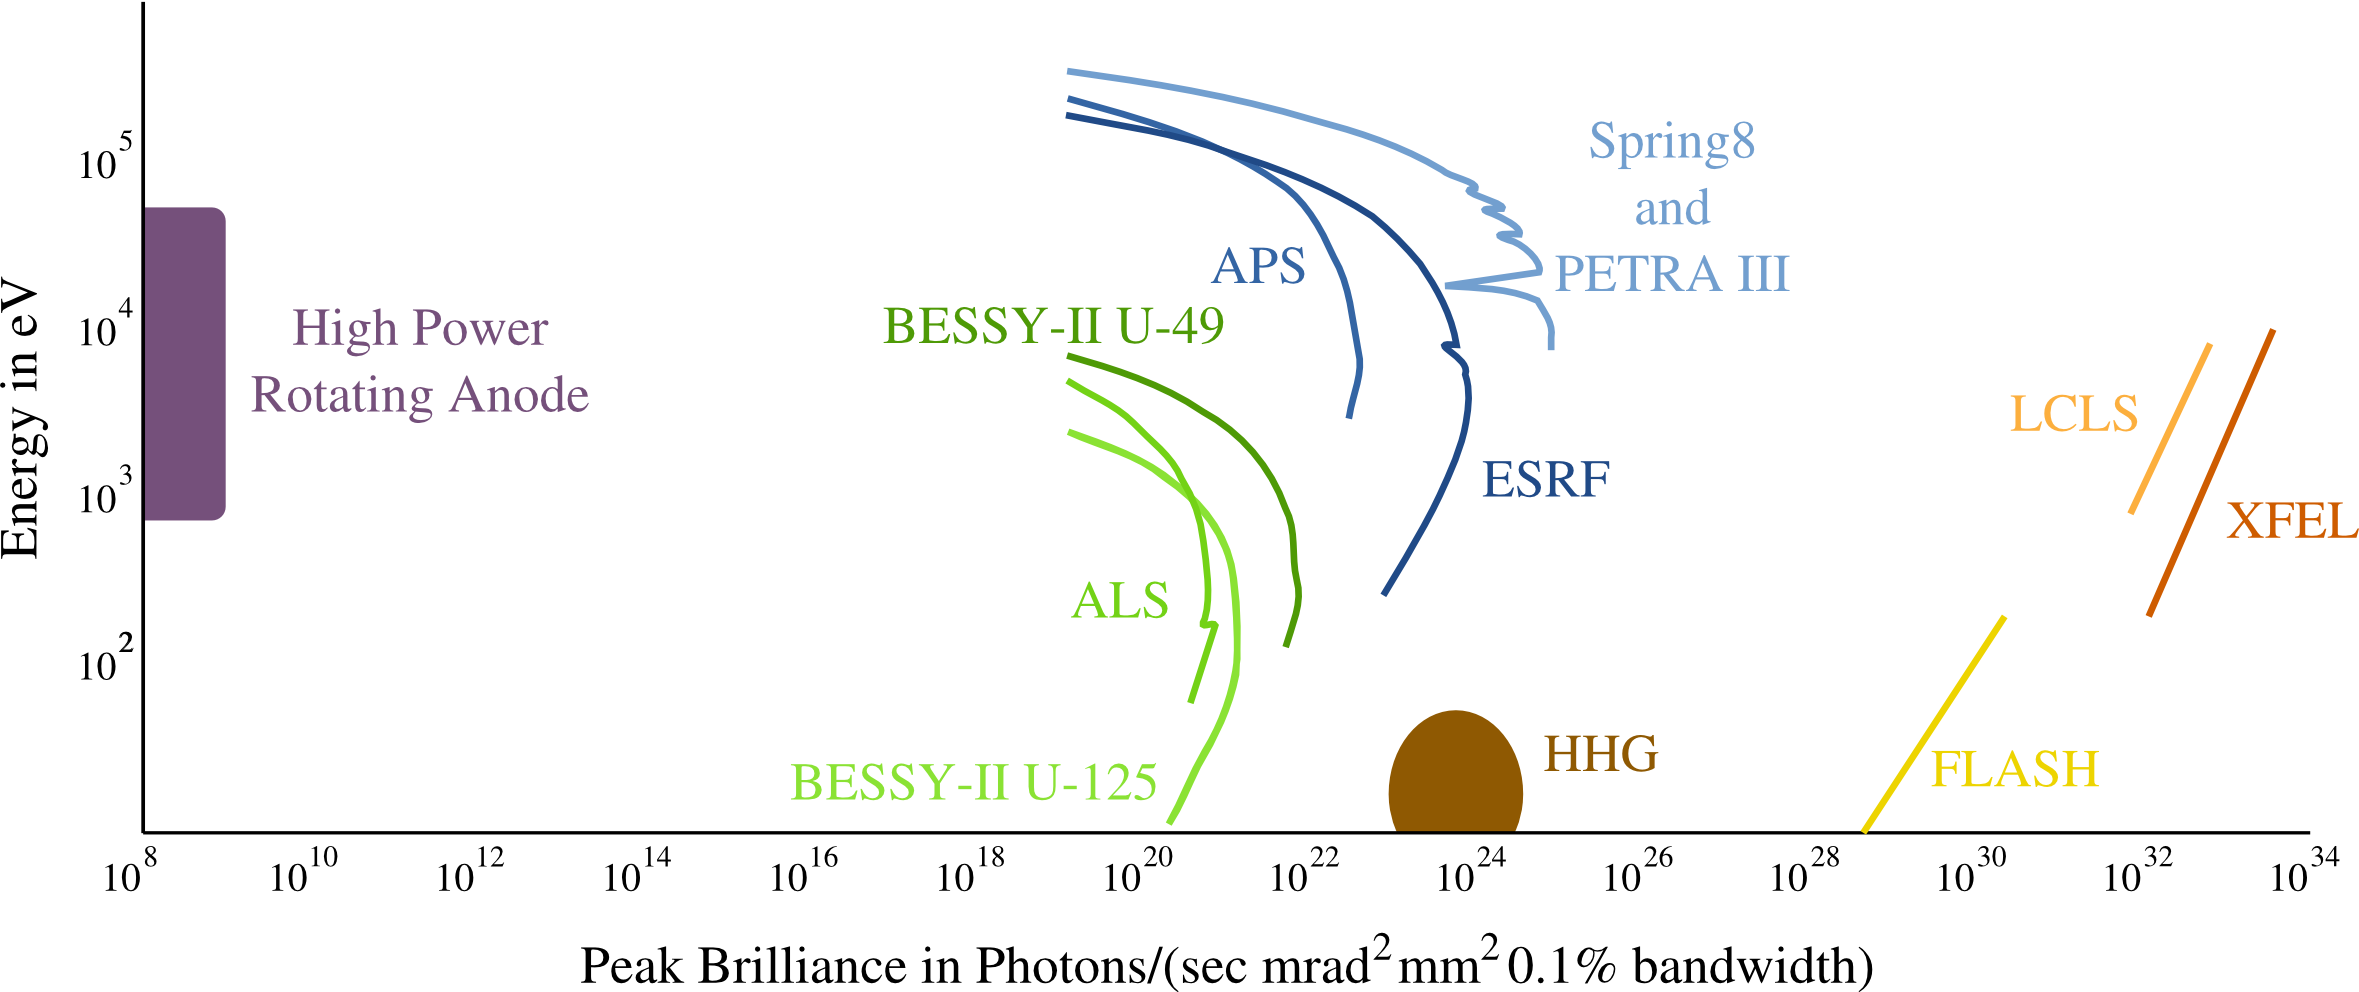
\includegraphics[width=1.0 \columnwidth]{brilliance.png}
  \caption{Peak brilliance of several X-ray sources. 
    Adapted from \cite{Ackermann2007Operation,Materlik2001TESLA}}
  \label{Fig:Brilliance}
\end{figure}

Yet the first dedicated synchrotron source (the SRS Daresbury) which began user
operation in 1981, produced just about 40 times higher beam intensities on the
sample than a laboratory X-ray generator. The synchrotron beam had better
coherence parameters, and it was tunable, but overall, the improvement was
evolutionary. X-ray lasers are different. The peak brightness of these lasers
exceeds present synchrotrons by $10^{10}$, the coherence degeneracy parameters exceed
synchrotrons by $10^9$, and the time resolution is $10^5$ times better. These
developments are extraordinary. The results will impact on a broad range of
disciplines, and guide technology and facility development in the future. 
 
%\section{X-ray lasers}
\section{Linear Accelerator-Driven Free-Electron Lasers}
 
A free-electron laser (FEL) is a parametric amplifier, which operates by
transferring energy to the output signal from an oscillator. An electron bunch
is accelerated to relativistic energies, and sent through a periodic magnetic
structure (undulator) where transverse oscillations and interference produce
synchrotron radiation enhanced at specific wavelengths. The intensity of this
radiation scales with the number of electrons in the bunch. Photons co-propagate
with the relativistic electrons and, if the undulator is long enough, induce an
energy modulation, leading to a periodic density modulation in the electron
cloud. The resulting microbunches behave like giant charged particles, and emit
photons proportional to the square of their total charge in the undulator. At
wavelengths longer than the bunch length, this radiation is coherent.

{\em Optically driven table-top X-ray lasers} use an intense optical laser pulse to
create coherent X-ray pulses in a plasma. The interaction of intense optical
fields with material at intensities of $10^{18}$ W/cm$^2$ and above is governed by the
electron relativistic behaviour, creating the domain of relativistic
optics. Electrons accelerated in such photon fields can be used in
ultra-brilliant X-ray sources, e.g. by laser-assisted synchrotron radiation,
linear and non-linear Compton scattering, betatron radiation or
free-electron-laser mechanisms. 
Currently these sources are not quite as powerful as FELs but
progress is fast, and table-top X-ray lasers may catch up with large linac-based
FELs. 

\begin{figure}[h]
\centering
  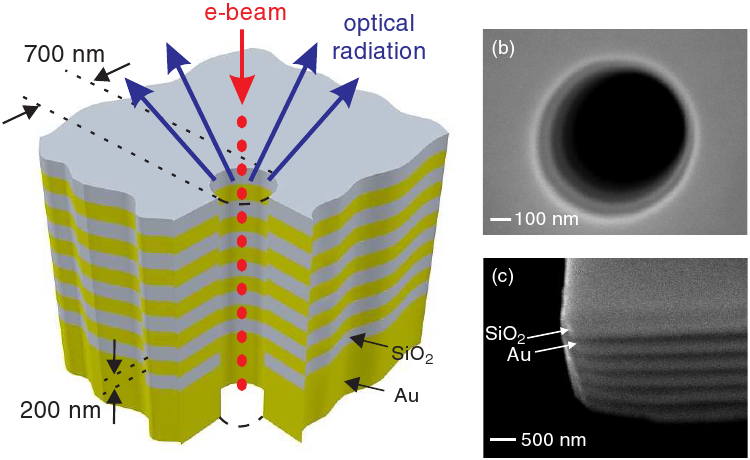
\includegraphics[width=0.6 \columnwidth]{FEL_on_a_chip.png}
  \caption{(a) Schematic cut-away section of a light
well, which comprises a nanohole through a stack of alternating
metal and dielectric layers, into which an electron beam is
launched. Light is generated as electrons travel down the well
and encounter a periodic material environment. (b) Scanning
electron microscope image of a light well fabricated in a gold-
silica multilayer. (c) The alternating metal-dielectric layer structure as seen
at an exposed corner of the sample. \cite{Adamo2009Light} 
}
\label{Fig:FEL_Chip}
\end{figure} 

X-ray lasers are bound to get smaller, more efficient and more affordable. A
recent paper describes a {\em free-electron laser on a chip}
(see Fig. \ref{Fig:FEL_Chip}). The tiny FEL utilises the Smith-Purcell effect
\cite{Smith1953Visible}, which is related to Cherenkov radiation.
  
There are signs that indicate that a major scientific explosion is taking shape.
 
% The introduction of free electron lasers brings with it an increase in peak
% brightness comparable to the change from rotating anodes to synchrotron sources
% (Fig. \ref{Fig:Brilliance}). They also offer very high coherence and ultra fast
% pulses of only a couple of femtoseconds opening a new window into the world of
% ultra fast science. HHG sources also shares many of the characteristics of free
% FELs albeit with lower peak power. In this chapter we will try to provide an
% overview of these two light sources.

% \section{Free electron lasers}

% Free electron lasers are in many ways a revolution from third generation
% synchrotrons and so they are often called fourth generation light sources. The
% fundamental difference between these two light sources is that while in a
% synchrotron photons are generated independently of each other in a free electron
% laser photon are generated in phase with each other and so cooperate to produce
% a pulse which has an intensity proportional to the square of the number of
% electrons being accelerated, instead of being linear with the number of
% electrons as is the case for a synchrotron.

\subsection{The SASE process}

The SASE process, central to all existing X-ray free electron lasers, is a
process in which the electrons are organized into micro bunches separated by the
distance of a wavelength, as they go through the undulator (see
Fig. \ref{Fig:Brilliance}). This happens because,
as in a normal synchrotron, when the electrons go through the undulator they
emit radiation due to the acceleration imposed by the magnetic field. If
the undulator is sufficiently long, this radiation starts to produce a
measurable effect in the distribution of the electrons making them accumulate in
micro bunches separated by exactly one wavelength. This is a self reinforcing
process as the more the electrons bunch together the stronger the field they
produce as they will radiate coherently. This process continues until almost all
the electrons are in these micro-bunches, at which point saturation is
reached. Under these conditions the microbunches behave like giant 
single particles and emit light proportional to the square of their total charge.

\begin{figure}[h]
\centering
  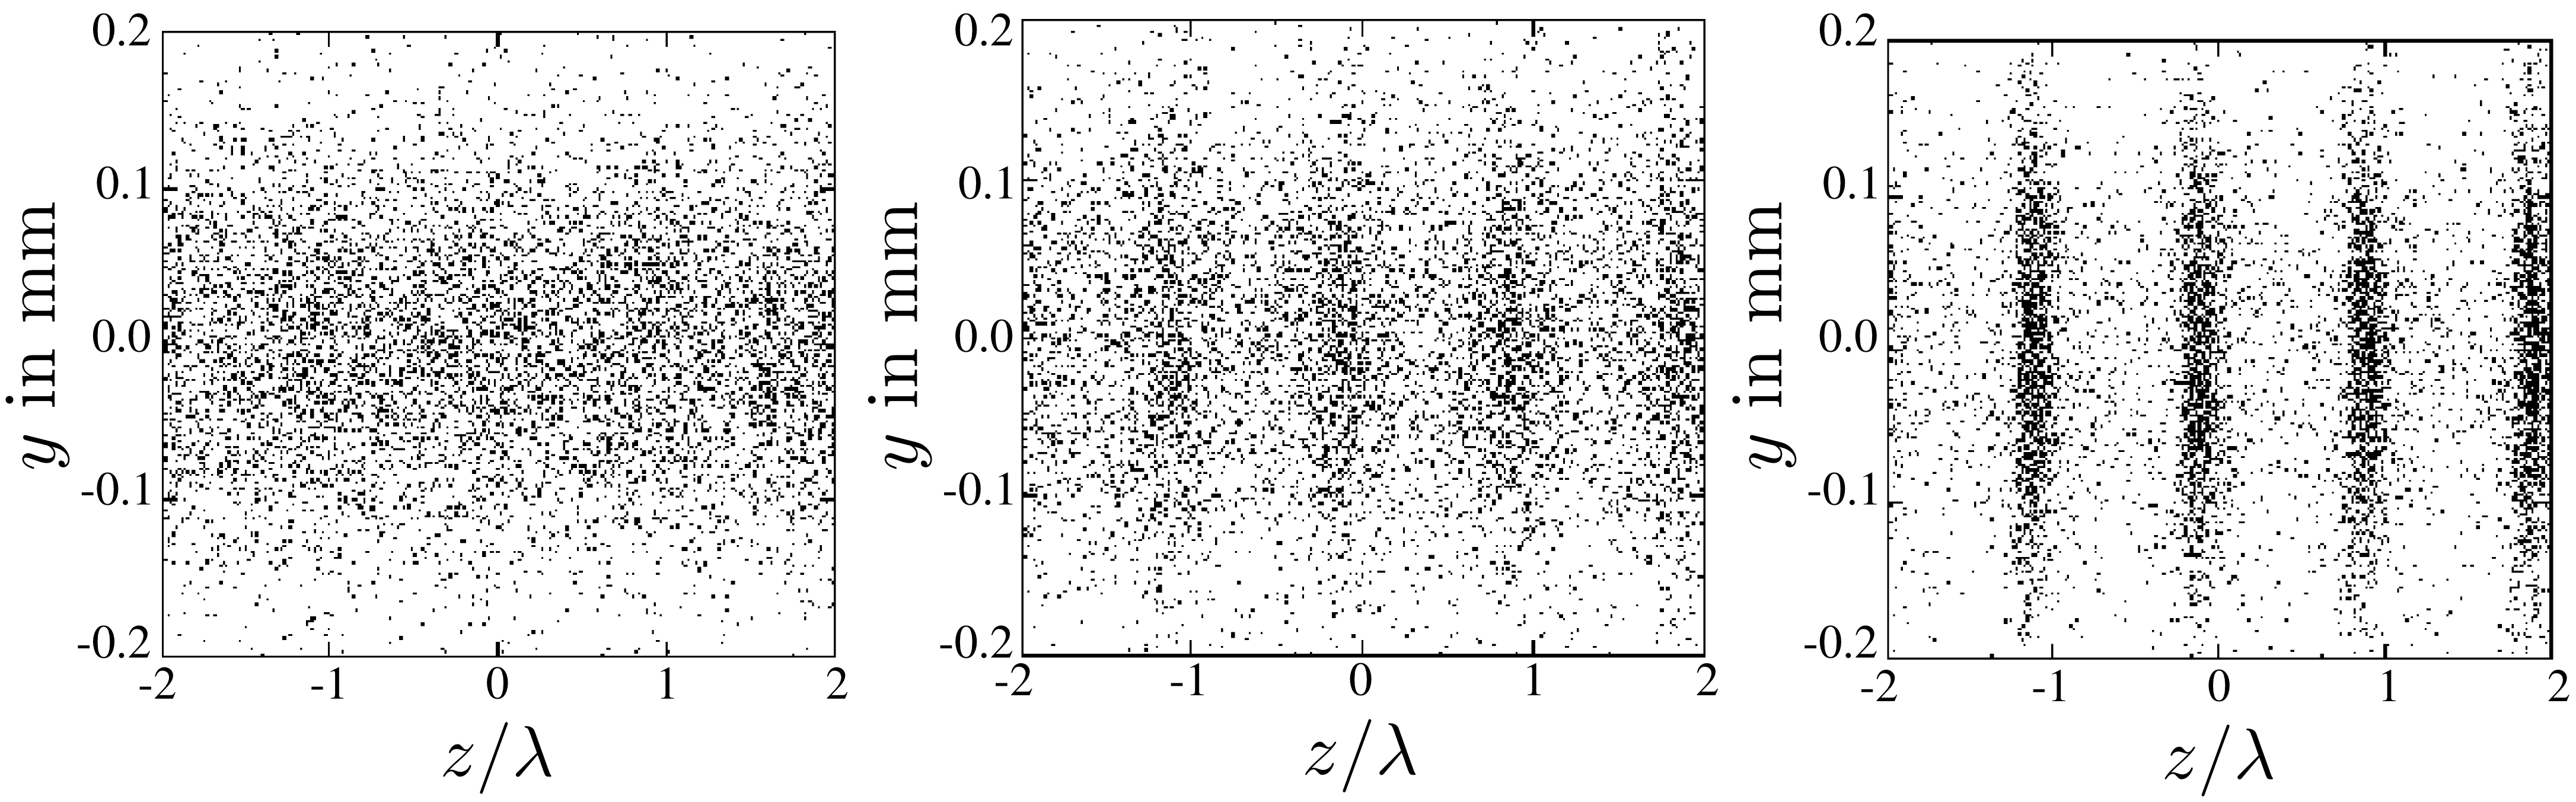
\includegraphics[width=1.0 \columnwidth]{micro-bunching.png}
  \caption{Simulation of micro-bunching during the SASE process where the
    electron density is represented by the density of dots. The snapshots
    from the left to the right represent the electron structure along the
    undulator, with the left side representing the beginning and the right side
    the end of the undulator. \cite{Materlik2001TESLA}}
  \label{Fig:Brilliance}
\end{figure}

The radiation produced by electrons distributed in this manner is much more
intense than if the electrons were uniformly distributed throughout the
undulator because with microbunching the distance between most of the electrons is
always a multiple of the wavelength, and so the radiated electric fields will be
in phase. In other words, the electrons radiate coherently and the resulting
intensity scales with the square of the number of electrons which is why the
difference in peak brilliance is so large.

\subsection{Current X-ray FEL Facilities}

X-ray FEL are developing at a very fast pace. The first hard X-ray FEL, the LCLS,
began user operations in October 2009.
% Nowadays there is only one hard X-ray FEL facility, LCLS at SLAC, USA and one
% one soft X-ray FEL named FLASH in DESY, Germany. 
There are several X-ray FELs
being built such as the European XFEL in Germany and SCSS
in Japan,
%both hard X-ray FEL
as well as several soft X-ray sources such as FERMI and SPARX
in Italy. The SwissFEL in Switzerland is also in planning stages. 
% Due to the fact that X-ray FEL use linear accelerators it is only
% possible to have beam in one beamline at the same time so even though the number
% of facilities is increasing quickly, access to an X-ray FEL will continue to be
% severely limited. 
The different characteristics of FEL radiation compared to a third generation synchrotron mean that while they are
often called fourth generation sources they will not replace synchrotrons in any
meaningful sense.
% as it happened in the past.
X-ray lasers should be considered a class of
their own better suited for other kinds of experiments than those possible at synchrotrons.

%\section{High harmonic generation}
\section{Optically-Driven Table-Top X-ray Lasers}

The first high harmonic generation (HHG) sources were created about two decades ago
and since then their power has been increasing as the power of all lasers usually
increases. They provide a relatively cheap and tunable source of very
short (a few fs) and intense pulses (more than $10^{10}$ photons per pulse). 

HHG works by shining a very intense optical laser into a gas. When the field of
the optical laser is sufficiently strong electrons in the gas will be ionized
by field ionization, and as the field progresses they will be accelerated back
towards the ion and finally recombine, generating in the process short
wavelength radiation (see Fig. \ref{Fig:HHG_Process}).

\begin{figure}[ht]
\centering
  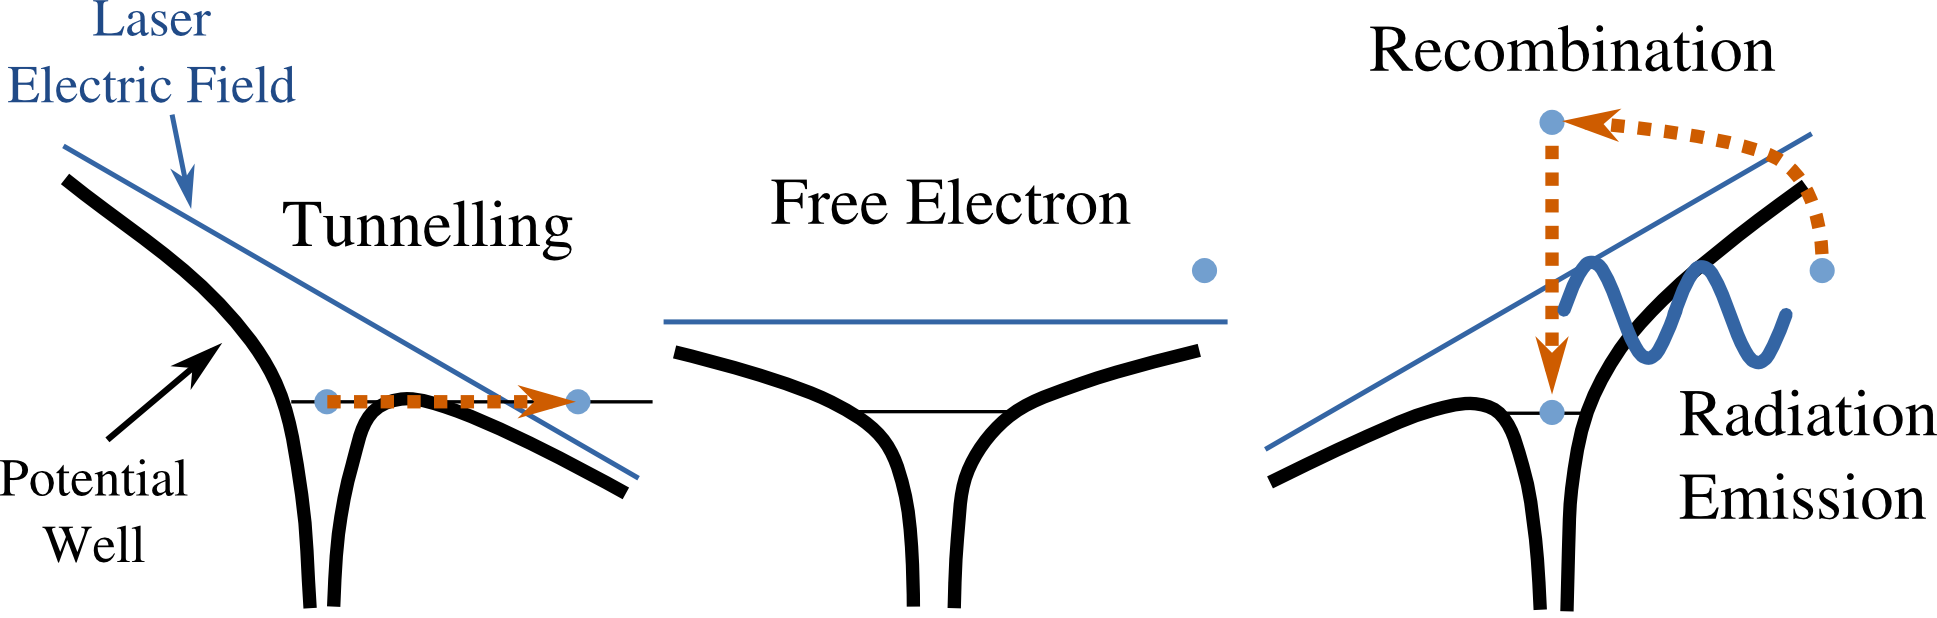
\includegraphics[width=1.0 \columnwidth]{HHG_Picture1.png}
  \caption{High harmonic generation process in an atom illuminated by an intense
    optical laser. The field is strong enough to distort the atomic potential
    well and allowing the electron to tunnel out. When the field reverses the
    electron is accelerated back towards the ion. Radiative recombination generates high
    energy radiation. \cite{Corkum1993Plasma,Lewenstein1994Theory}}
  \label{Fig:HHG_Process}
\end{figure}

% * High Harmonic Generation

% - Started one decade ago
% - Short description with non linear effects
% - Show some scheme of the setup
% - Very short pulse lengths
% - 
%%% Local Variables: 
%%% mode: latex
%%% TeX-master: "Thesis"
%%% End: 
